%\documentclass[12pt,a4paper,numbers=noenddot,bibliography=totocnumbered,listof=totocnumbered]{scrartcl}

\documentclass[ fontsize=12pt,
				a4paper,
				twoside,
				openright,
				DIV=10,
				pagesize,
				bibliography=totoc,
				listof=totoc,
				titlepage,
				draft=false,
				parskip=true,
				dvipsnames]
				{scrreprt}
				
%-------------------------------------
% Stichpunkte
%
% i: punktuell (\item ...)
% e: nummeriert (\item ...)
% d: fett (\item[...]) mit Beschreibung dahinter
%-------------------------------------
\newcommand\numberthis{\addtocounter{equation}{1}\tag{\theequation}}

% --- Punktuell
\newcommand{\bi}{\begin{itemize}}
\newcommand{\ei}{\end{itemize}}

% --- Nummeriert
\newcommand{\be}{\begin{enumerate}}
\newcommand{\ee}{\end{enumerate}}

% --- Fettgeschrieben mit Beschreibung
\newcommand{\bd}{\begin{description}}
\newcommand{\ed}{\end{description}}



%-------------------------------------
% Sonderzeichen
% 
% „...“:	\gqq{...}
%-------------------------------------

\newcommand{\gqq}[1]{{\glqq}#1{\grqq}}



%-------------------------------------
% Firmen- und Marken-Namen
% 
% Firma [kursiv]:		\firma{...}
% Produktname [kursiv]:	\produkt{...}
% Marke [Kapitälchen]:	\marke{...}
%-------------------------------------

\newcommand{\firma}[1]{\textit{#1}}
\newcommand{\produkt}[1]{\textit{#1}}
\newcommand{\marke}[1]{\textsc{#1}}



%-------------------------------------
% Fußnote auf andere Fußnote referenziert
%
% \footnote{text\label{xy}}
% \ftnref{xy}
%-------------------------------------

\newcommand\ftnref[1]{\textsuperscript{\ref{#1}}}



%-------------------------------------
% Quelle am Ende eines Kapitels
%
% Quelle: ... 	= 	\quelle{...}
% Quellen: ... 	= 	\quellen{...}
%-------------------------------------

\newcommand\quelle[1]{\begin{footnotesize}\textit{Quelle: #1}\end{footnotesize}}
\newcommand\quellen[1]{\begin{footnotesize}\textit{Quellen: #1}\end{footnotesize}}
\usepackage{mathtools}
\usepackage{siunitx}
\usepackage{rotating}
\usepackage{adjustbox}
\usepackage{blindtext}

\DeclarePairedDelimiter\ceil{\lceil}{\rceil}

%Text
	\usepackage[utf8]{inputenc} 						%UTF-8 Encoding
	\usepackage{microtype}								%Typographieoptimierung (erst vorm Druck einkommentieren, DAUERT SEEEEEHR LANGE)
	\usepackage[ngerman]{babel}							%Textsprache Deutsch
	\usepackage{amssymb}								%Zusätzliche Symbole
	\usepackage{textgreek}								%Griechische Zeichen im Fließtext (ohne Mathemodus)

%Grafiken
	\usepackage{graphicx}								%Einbinden von Bildern
	\usepackage{wrapfig}								%Bilder von Text umflossen
	\usepackage{subfig}									%Mehrere Bilder in einer Abbildung
%	\usepackage{svg}									%Einbingen von SVG-Vektorgrafiken (benötigt vollständige Installation von Inkscape!)
	\usepackage{xcolor}									%Zusätzliche Farben
	\usepackage{transparent}							%

%Tabellen
	\usepackage{longtable}								%Tabelle über mehrere Seiten
	\usepackage{tabularx}								%Tabelle mit fixer Breite und variabler Spaltenbreite
	\newcolumntype{Y}{>{\centering\arraybackslash}X}	%Neuer Spaltentyp f. TabularX: Y == zentriert X
	\newcolumntype{R}{>{\raggedleft\arraybackslash}X} 	%Neuer Spaltentyp f. TabularX: R == rechtsbündig X
	\usepackage{multirow}
	\usepackage{caption}

\renewcaptionname{ngerman}{\figurename}{Abb.}
\renewcaptionname{ngerman}{\tablename}{Tab.}

%Misc
	\PassOptionsToPackage{hyphens}{url}					%URLs umbrechen an Bindestrichen
	%\usepackage[colorlinks=true]{hyperref}				%Klickbare Links in PDF in Farbe und Bunt. 
	\usepackage{hyperref}								%Klickbare Links in PDF (farbige Ausgabe unterdrückt, roter Kasten um Links)
	\usepackage{pdfpages} 								%mehrseitige PDFs einbinden
	\usepackage[printonlyused]{acronym}					%Abkürzungsverzeichnis ([printonlyused] gibt nur benutzte Abkürzungen aus)
	\usepackage{nameref}								%Referenz auf Name (z.B. Kapitelname)
	\usepackage{eurosym}								%€-Symbol per \EUR
	\usepackage[numbers,square]{natbib}					%Erweitertes bibtex, Nummern in eckigen Klammern
	\usepackage{listings}								%Quellcode-Listings einfügen
		\lstloadlanguages{Python,[Sharp]C}				%Laden der verwendeten Programmiersprachen
	\usepackage{scrhack}
	\usepackage[ngerman]{todonotes}						%ToDo Notizen und Liste der ToDos 
	\usepackage{chngcntr}
		\counterwithout{footnote}{chapter}				%Fußnoten werden global nummeriert, nicht mehr je Kapitel
	\usepackage{appendix}								%Anhangorganisation
%	\usepackage[open]{bookmark}							%Öffne Lesezeichen in der PDF-Anzeige


%Textsatz
	\clubpenalty10000									%Hurenkinder und Schusterjungen verhindern
	\widowpenalty10000
	\displaywidowpenalty=10000


%%%%%%%%%%%%%%%%%%%%%%%%%%%%%%%%%%%%%%%%%%%%%%%%%%%%%%%%%%%%%%%%%%%%%%%%%%

\usepackage{amsmath}
\usepackage{amsfonts}
\usepackage{amssymb}
\usepackage{fancyhdr}
\usepackage{geometry}
\usepackage{setspace}
\usepackage{floatflt}
\usepackage{colortbl}
\usepackage{paralist}
\usepackage{array}
\usepackage{parskip}
\usepackage[subfigure,titles]{tocloft}

\makeatletter
\def\l@lstlisting#1#2{\@dottedtocline{1}{0em}{1em}{\hspace{1,5em} Lst. #1}{#2}}
\makeatother

%%%% Global Variables

%%%%%%%%%%%% personal data %%%%%%%%%%%%
%% persons and stuff
% the name of the author
\def \GlobalsAuthorName
{Max Mustermann}
% the email address of the author
\def \GlobalsAuthorMail
{MaMu1111@hs-karlsruhe.de}
% the matr-nr of the author
\def \GlobalsAuthorMatrikelNr
{11111}
% the name of the first referent
\def \GlobalsReferentName
{Prof. Dr.-Ing. Max Mustermann}
% the name of the second referent
\def \GlobalsCoreferentName
{Prof. Dr. rer. nat. Max Mustermann}
% the name of the Betreuer in der Firma
\def \GlobalsBetreuerName
{Dip. Ing. Leo, Max Mustermann}
% the name of the company
\def \GlobalsCompanyName
{Firmenname}
% the adress of the company
\def \GlobalsCompanyAdress
{Musterstraße 1 \newline 11111 Musterstadt}
% the deadline of the thesis
\def \GlobalsDeadlineDate
{01.01.1911}

%% institutions and stuff
% the path of the picture which shall be embedded at the left top of the title page
\def \GlobalsCollegePicturePath
{50_Bilder/hs_logo.png}
% the path of the picture which shall be embedded at the right top of the title page
\def \GlobalsFacultyPicturePath
{50_Bilder/faculty_logo.png}
% the name of the faculty
\def \GlobalsFacultyName
{Elektro- und Informationstechnik}
% the title of the thesis
\def \GlobalsThesisTitle
{Überschrift des Themas}
% this describes what kind of work you are doing, and why.
\def \GlobalsWhatKindOfWork
{Wissenschaftliche Arbeit zur Erlangung des Grades \\  Master of Science  (M. Sc.) im Studiengang Automatisierungstechnik \\ an der Hochschule Karlsruhe - Technik und Wirtschaft}
% what is it? bachelor thesis, master thesis, project work?
\def \GlobalsSortOfName
{Masterarbeit (M. Sc.)}

%%%%%%%%%%%%%%%%%%%%%%%%%%%%%%%%%%%%%%%%%%%%%%%%%%%%%%%%%%%%%%%%%%%%%%%%%%%%%%%%%

%%% Variables for the side edges (Übernommen aus den Hinweisen zu Abschlussarbeiten von Herr Arnemann)
% space to top of the page
\def \GlobalsGeometryTop
{25mm}
% space to left of the page
\def \GlobalsGeometryLeft
{30mm}
% space to right of the page
\def \GlobalsGeometryRight
{30mm}
% space to bottom of the page
\def \GlobalsGeometryBottom
{40mm}
% the distance between head and content
\def \GlobalsGeometryHeadsep
{12mm}
% the distance between content and footer
\def \GlobalsGeometryFootskip
{12mm}

\geometry{
	a4paper,
	top=\GlobalsGeometryTop,
	left=\GlobalsGeometryLeft,
	right=\GlobalsGeometryRight,
	bottom=\GlobalsGeometryBottom,
	headsep=\GlobalsGeometryHeadsep,
	footskip=\GlobalsGeometryFootskip}

\hypersetup{
	unicode=false, pdftoolbar=true, pdfmenubar=true, pdffitwindow=false, pdfstartview={FitV},
    pdftitle={\GlobalsSortOfName},
    pdfauthor={\GlobalsAuthorName},
    pdfsubject={Konzeption und Implementierung einer Schnittstelle zwischen zwei Cloud-Anbietern},
    pdfcreator={\LaTeX\ with package \flqq hyperref\frqq},
    pdfproducer={pdfTeX \the\pdftexversion.\pdftexrevision},
    pdfkeywords={\GlobalsSortOfName; Hochschule Karlsruhe; Automatisierungstechnik; AXOOM; Cloud; Azure; Industrie 4.0},
    pdfnewwindow=true}
%    colorlinks=true,linkcolor=black,citecolor=black,filecolor=magenta,urlcolor=black	%kein roter Rahmen um Links
    
\pdfinfo{/CreationDate (D:20180102133321)}


\setkomafont{caption}{\small}





\begin{document}

\pagestyle{headings}

% ----------------------------------------------------------------------------------------------------------
% ----------------------------------------------------------------------------------------------------------
% ### Vorspann ###
\pagenumbering{roman}

% ----------------------------------------------------------------------------------------------------------
% Titelseite Version 1 und 2
\thispagestyle{empty}

\begin{center}

\begin{table}[h!]
\hspace{-1cm}
\begin{tabular}{m{0.6\textwidth}c}
  \includegraphics[width=0.4\textwidth]{\GlobalsCollegePicturePath} &  \includegraphics[width=0.4\textwidth]{\GlobalsFacultyPicturePath} 
	\end{tabular}
	\vspace*{2cm}
\end{table}

%	\Large
%	\textbf{Fakultät für}\\
%	\textbf{\GlobalsFacultyName}\\
%	\vspace*{2cm}

	\Large
	\textbf{\GlobalsThesisTitle}\\
	\vspace*{0.5cm}

	\normalsize
	%über das Thema\\
	\vspace*{1.5cm}
	\textbf{Masterarbeit (M. Sc.)} \\
	\vspace*{0.5cm}
	\GlobalsWhatKindOfWork\\
%	\vspace*{1cm}

	\vfill
	\normalsize
	\newcolumntype{x}[1]{>{\raggedleft\arraybackslash\hspace{0pt}}p{#1}}
	\begin{tabular}{x{4cm}p{7.5cm}}
	
		\rule{0mm}{5ex}\textbf{Autor:} & 	\GlobalsAuthorName \newline
											Matrikel-Nr. \GlobalsAuthorMatrikelNr \newline
											\GlobalsAuthorMail \\
											
		\rule{0mm}{5ex}\textbf{Referent:} & \GlobalsReferentName \\
		
		\rule{0mm}{5ex}\textbf{Korreferent:} & \GlobalsCoreferentName \\
		
		\rule{0mm}{5ex}\textbf{Betreuer (Firma):} & \GlobalsBetreuerName \\
		
		\rule{0mm}{5ex}\textbf{Unternehmen:} & 	\GlobalsCompanyName \newline
												\GlobalsCompanyAdress \\
		
		\rule{0mm}{5ex}\textbf{Abgabe:} & \GlobalsDeadlineDate \\
		
	\end{tabular}
	
\end{center}

\newpage
\thispagestyle{empty}
~
\newpage

% ----------------------------------------------------------------------------------------------------------
% Aufgabenstellung
\thispagestyle{empty}
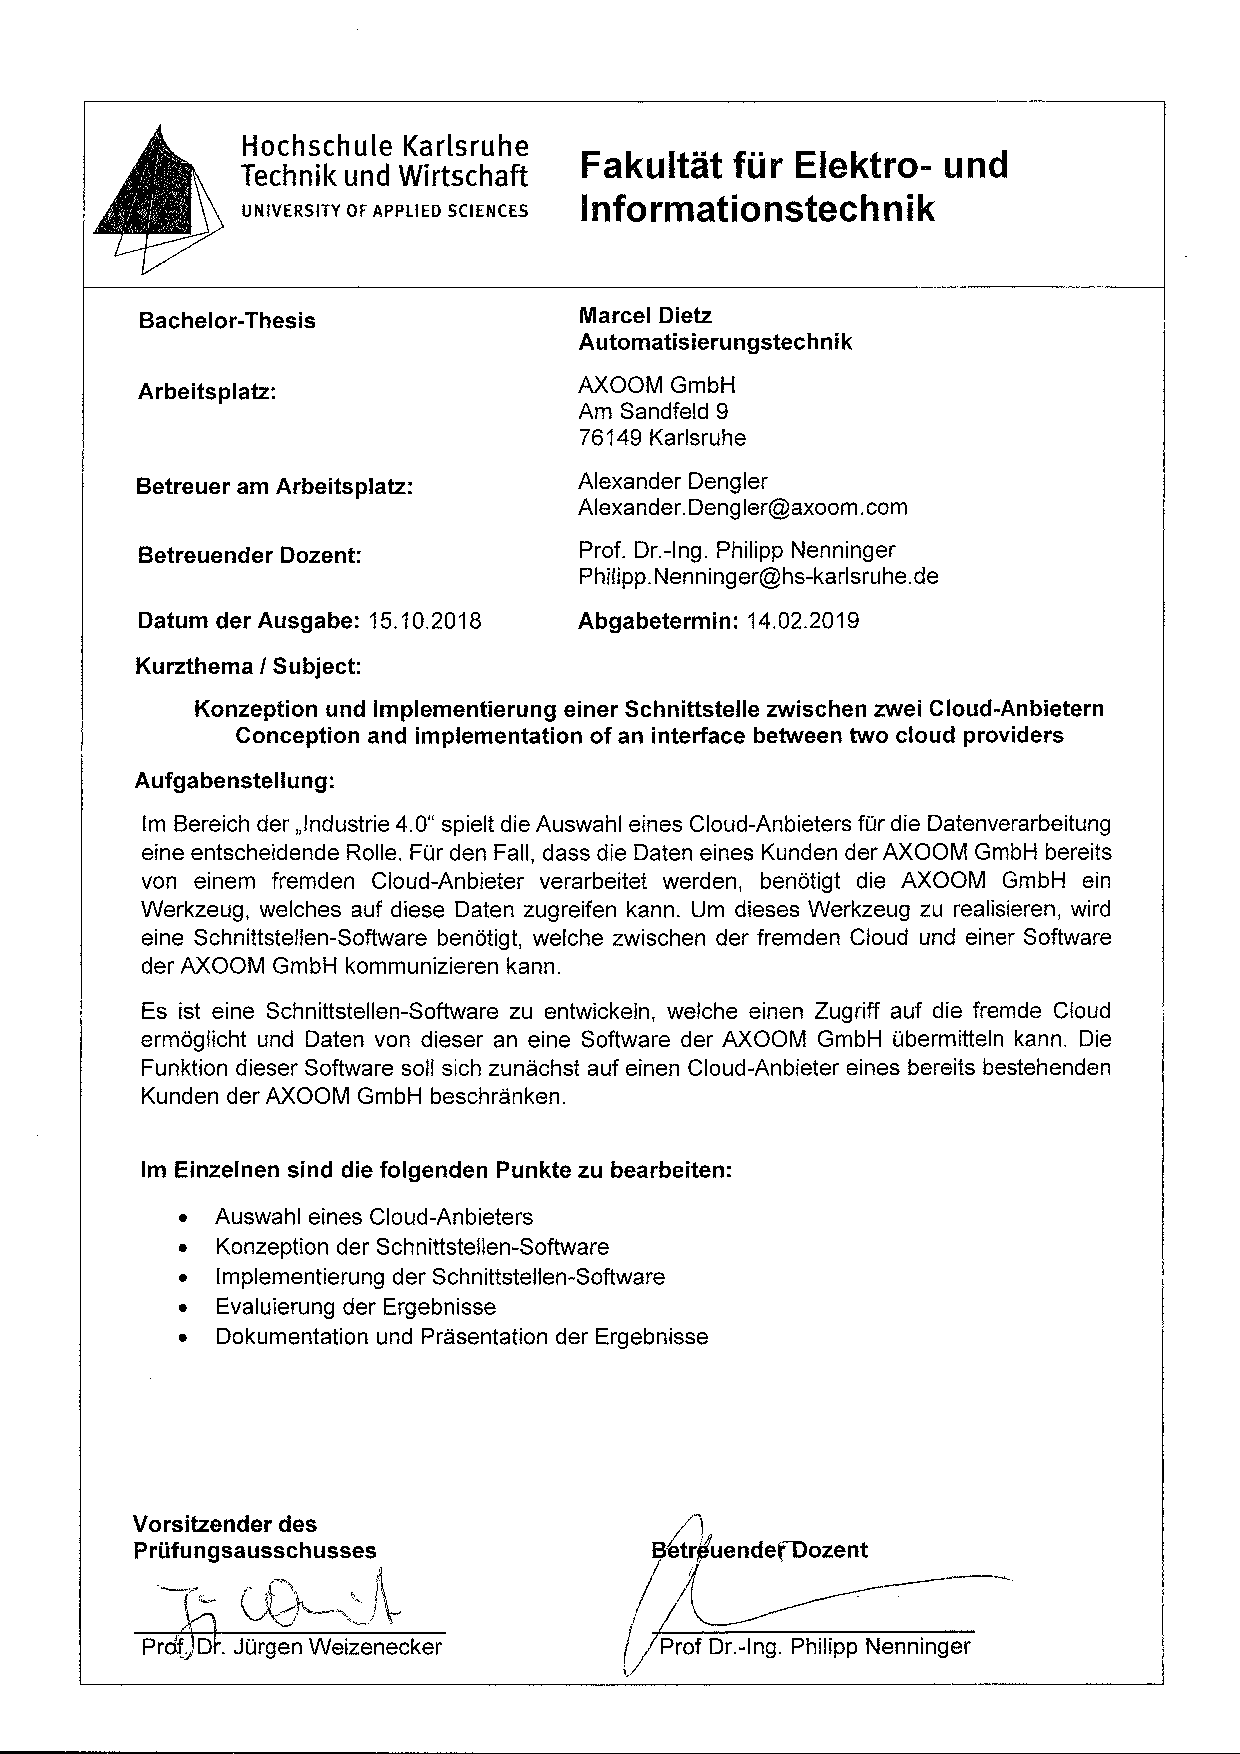
\includepdf{60_Include/Aufgabenstellung.pdf}
\pagebreak

% ----------------------------------------------------------------------------------------------------------
% Sperrvermerk
\chapter*{\centerline{Sperrvermerk}}\label{chap:Sperrvermerk}

Die vorliegende Arbeit wurde von Max Mustermann, wohnhaft in der Musterstraße 1, 11111 Musterstadt erstellt. Sie beinhaltet vertrauliche Informationen der \firma{Firmenname}.

Die Weitergabe des Inhaltes und beiliegender Daten im Gesamten oder in Teilen ist grund\-sätz\-lich untersagt. Es dürfen keinerlei Kopien oder Abschriften -- auch in digitaler Form -- angefertigt werden. Ausnahmen bedürfen der vorherigen ausdrücklichen schriftlichen Genehmigung durch den Verfasser und der Firma.

\vspace*{2cm}

\hfill Musterstadt, den 1. Januar 1911, ~ \rule{0.3\textwidth}{0.4pt}

\hfill\parbox{0.20\textwidth}{\footnotesize{Max Mustermann}}

\newpage
\thispagestyle{empty}
~
\newpage

% ----------------------------------------------------------------------------------------------------------
% Erklärung
\chapter*{\centerline{Eigenständigkeitserklärung}}\label{chap:Erklaerung}

Ich versichere hiermit, dass ich die nachfolgende Arbeit mit dem Thema: \gqq{\produkt{Themenüberschrift}} selbstständig und ohne fremde Hilfe verfasst und keine anderen als die im Literaturverzeichnis angegebenen Hilfsmittel verwendet habe. Insbesondere versichere ich, dass ich alle wörtlichen und sinngemäßen Übernahmen aus anderen Werken als solche kenntlich gemacht und mit genauer Quellenangabe dargelegt habe. Die Arbeit hat mit gleichem Inhalt bzw. in wesentlichen Teilen noch keiner anderen Prüfungsbehörde vorgelegen.

\vspace*{2cm}

\hfill Musterstadt, den 1. Januar 1911, ~ \rule{0.3\textwidth}{0.4pt}

\hfill\parbox{0.20\textwidth}{\footnotesize{Max Mustermann}}

\newpage
\thispagestyle{empty}
\chapter*{\centerline{Geschlechtergerechte Sprache}}

Der besseren Lesbarkeit halber wird in dieser wissenschaftlichen Arbeit in der Regel die Sprachform des generischen Maskulinums angewendet. Es wird an dieser Stelle darauf hingewiesen, dass die ausschließliche Verwendung der männlichen Form geschlechtsunabhängig verstanden werden soll.
\newpage
\thispagestyle{empty}
~
\newpage

% ----------------------------------------------------------------------------------------------------------
% Danksagung
\chapter*{\centerline{Danksagung}}\label{chap:Danksagung}

% Anregungen, Literaturhinweise, Formatieren, Korrekturlesen, Finanzielle Unterstützung

An dieser Stelle möchte ich mich bei all jenen bedanken, die durch ihre fachliche und persönliche Unterstützung zum Erfolg meiner Bachelorarbeit beigetragen haben.

\blindtext

\newpage
\thispagestyle{empty}
~
\newpage


% ----------------------------------------------------------------------------------------------------------
% Kurzfassung
\chapter*{\centerline{Kurzfassung}}\label{chap:Kurzfassung}
%native language, max. 1 page

%
\blindtext



\newpage
\thispagestyle{empty}
~
\newpage

\chapter*{\centerline{Abstract}}\label{chap:Abstract}
%Englisch, max. 1 page
\blindtext




\newpage
\thispagestyle{empty}
~
\newpage

% ----------------------------------------------------------------------------------------------------------
% Inhaltsverzeichnis
\tableofcontents

% ----------------------------------------------------------------------------------------------------------
% ----------------------------------------------------------------------------------------------------------
% ### Inhalt ###
% ----------------------------------------------------------------------------------------------------------
% Kapitel 1 - Einleitung
\chapter{Einleitung}\label{chap:Einleitung}
\pagenumbering{arabic}
\setcounter{page}{1}
\blindtext

\section{Unternehmensvorstellung}\label{sec:1_Firma}

\textit{\textbf{Die Informationen im Folgenden stammen aus firmeninternen Quellen.}}\\

\blindtext

\blindtext

\newpage

\section{Motivation}\label{sec:1_Motivation}

\blindtext

\blindtext

\blindtext

\newpage
\section{Aufgabenstellung}\label{sec:1_Aufgabenstellung}

\blindtext

\newpage
\section{Aufbau der Arbeit}\label{sec:1_AufbauArbeit}

\blindtext

\newpage


% ----------------------------------------------------------------------------------------------------------
% Kapitel 2 - Grundlagen
\chapter{Konzept}\label{chap:Konzept}

\blindtext

% ----------------------------------------------------------------------------------------------------------
% Kapitel 3 - Stand der Technik
\input{20_Inhalt/23-Stand_der_Technik.tex}

% ----------------------------------------------------------------------------------------------------------
% Kapitel 4 - Konzept
\input{20_Inhalt/24-Konzeption.tex}
% Einfügen eines Seitenumbruchs im Inhaltsverzeichnis
\addtocontents{toc}{\protect\newpage}

% ----------------------------------------------------------------------------------------------------------
% Kapitel 5 - Implementierung
\input{20_Inhalt/25-Implementierung.tex}

% ----------------------------------------------------------------------------------------------------------
% Kapitel 6 - Evaluation und Tests
\input{20_Inhalt/26-Evaluation_und_Test.tex}

% ----------------------------------------------------------------------------------------------------------
% Kapitel 7 - Zusammenfassung und Ausblick
\input{20_Inhalt/27-Zusammenfassung_und_Ausblick.tex}

% ----------------------------------------------------------------------------------------------------------
% ----------------------------------------------------------------------------------------------------------
% ### Abspann ###
\pagestyle{empty}

% ----------------------------------------------------------------------------------------------------------
% Verzeichnisse
\chapter*{Abkürzungsverzeichnis}

\pagenumbering{Roman}

\addcontentsline{toc}{chapter}{Abkürzungsverzeichnis}

\begin{acronym}[XAML] % längste Abkürzung steht in eckigen Klammern

	\setlength{\itemsep}{-\parsep} % geringerer Zeilenabstand
	
%123
	\acro{3D}{dreidimensional\acroextra{; hier: räumliche Darstellung}}
%A
	\acro{App}{Application\acroextra{, dt.: Anwendungssoftware}}
	\acro{AWS}{Amazon Web Service}
	\acro{API}{Application Programming Interface\acroextra{, dt.: Programmierschnittstelle}}
	\acro{ASCII}{American Standard Code for Information Interchange}
%B
	%\acro
%C
	%\acro
%D
	%\acro
%E
	%\acro
%F
	%\acro
%G
	%\acro
%H
	%\acro
%I
	%\acro
%J
	%\acro
%K
	%\acro
%L
	%\acro
%M
	%\acro
%N
	%\acro
%O
	%\acro
%P
	%\acro
%Q
	%\acro
%R
	%\acro
%S
	%\acro
%T
	%\acro
%U
	%\acro
%V
	%\acro
%W
	%\acro
%X
	%\acro
%Y
	%\acro
%Z
	%\acro
	
\end{acronym}

\newpage
% TODO Typ vor Nummer
\renewcommand{\cfttabpresnum}{Tab. }
\renewcommand{\cftfigpresnum}{Abb. }
\settowidth{\cfttabnumwidth}{Abb. 10\quad}
\settowidth{\cftfignumwidth}{Abb. 10\quad}

\begin{footnotesize}

% --- Abbildungsverzeichnis
%\rhead{VERZEICHNISSE}
\listoffigures
\newpage

% --- Tabellenverzeichnis
\listoftables
\newpage

%% --- Listing-Verzeichnis
%\renewcommand{\lstlistlistingname}{Listing-Verzeichnis}
%\lstlistoflistings
%%{\labelsep2cm\lstlistoflistings}
%\newpage

\end{footnotesize}

% --- Literaturverzeichnis
\bibliographystyle{unsrtdin}	%natdin %dinat %unsrtdin
\bibliography{30_Verzeichnisse/biblio.bib}
\newpage




% ----------------------------------------------------------------------------------------------------------
% Literatur (verwendete Literatur)
% ----------------------------------------------------------------------------------------------------------
%\renewcommand\refname{Literaturverzeichnis}
%\addcontentsline{toc}{chapter}{Literaturverzeichnis}
%\bibliographystyle{plain}
%\bibliography{30_Anhang/31_Literaturverzeichnis}
%\newpage

% ----------------------------------------------------------------------------------------------------------
% Anhang
%\pagenumbering{Roman}
%\setcounter{page}{1}
%\lhead{Anhang \thesection}

\appendix
\renewcommand{\appendixtocname}{Anhang}
\renewcommand{\appendixname}{Anhang}
\renewcommand{\appendixpagename}{Anhang}
\renewcommand*{\thesection}{Anhang \Alph{section}}
\renewcommand{\thefigure}{\Alph{section}.\arabic{figure}}
\renewcommand{\thetable}{\Alph{section}.\arabic{table}}
\addappheadtotoc
\appendixpage

\addtocontents{toc}{\protect\setcounter{tocdepth}{-1}}

\begin{figure}[ht]
  \begin{adjustbox}{addcode={\begin{minipage}{\width}}{\caption[Bildname 1 \newline (Quelle: Google.de)]{%
      Bildname 1 der \firma{Firma}
      }\label{abb:Anhand1}\end{minipage}},rotate=90,center}
	
\includegraphics[width=1.3\textwidth]{40_Anhang/Folder1/Picture1.PNG}
  \end{adjustbox}
\end{figure}

\newpage


\end{document}
